%%%%%%%%%%%%%%%%%%%%%%%%%%%%%%%%%%%%%
%                                   %
% Compile with XeLaTeX and biber    %
%                                   %
% Questions or comments:            %
%                                   %
% joshua dot mcneill at uga dot edu %
%                                   %
%%%%%%%%%%%%%%%%%%%%%%%%%%%%%%%%%%%%%

\documentclass{beamer}
  % Read in standard preamble (cosmetic stuff)
  %%%%%%%%%%%%%%%%%%%%%%%%%%%%%%%%%%%%%%%%%%%%%%%%%%%%%%%%%%%%%%%%
% This is a standard preamble used in for all slide documents. %
% It basically contains cosmetic settings.                     %
%                                                              %
% Joshua McNeill                                               %
% joshua dot mcneill at uga dot edu                            %
%%%%%%%%%%%%%%%%%%%%%%%%%%%%%%%%%%%%%%%%%%%%%%%%%%%%%%%%%%%%%%%%

% Beamer settings
% \usetheme{Berkeley}
\usetheme{CambridgeUS}
% \usecolortheme{dove}
% \usecolortheme{rose}
\usecolortheme{seagull}
\usefonttheme{professionalfonts}
\usefonttheme{serif}
\setbeamertemplate{bibliography item}{}

% Packages and settings
\usepackage{fontspec}
  \setmainfont{Charis SIL}
\usepackage{hyperref}
  \hypersetup{colorlinks=true,
              allcolors=blue}
\usepackage{graphicx}
  \graphicspath{{../../figures/}}
\usepackage[normalem]{ulem}
\usepackage{enumerate}

% Document information
\author{M. McNeill}
\title[FREN2001]{Français 2001}
\institute{\url{joshua.mcneill@uga.edu}}
\date{}

%% Custom commands
% Lexical items
\newcommand{\lexi}[1]{\textit{#1}}
% Gloss
\newcommand{\gloss}[1]{`#1'}
\newcommand{\tinygloss}[1]{{\tiny`#1'}}
% Orthographic representations
\newcommand{\orth}[1]{$\langle$#1$\rangle$}
% Utterances (pragmatics)
\newcommand{\uttr}[1]{`#1'}
% Sentences (pragmatics)
\newcommand{\sent}[1]{\textit{#1}}
% Base dir for definitions
\newcommand{\defs}{../definitions}


  % Packages and settings
  \usepackage[style=apa, backend=biber]{biblatex}
    \addbibresource{../references/References.bib}

  % Document information
  \subtitle[Speech Perception]{Speech Perception}

  %% Custom commands
  % Subsection/frame titles
  \newcommand{\suboneone}{What are we doing?}
  \newcommand{\subonetwo}{Normalization}
  \newcommand{\subonethree}{Categorical perception}
  \newcommand{\subonefour}{Linguistic context}
  \newcommand{\subonefive}{Speech rate}
  \newcommand{\subonesix}{The McGurk effect}
  \newcommand{\suboneseven}{Mental grammar and lexicon}
  \newcommand{\suboneeight}{Phonemic restoration}
  \newcommand{\subonenine}{Practice}

\begin{document}
  % Read in the standard intro slides (title page and table of contents)
  %%%%%%%%%%%%%%%%%%%%%%%%%%%%%%%%%%%%%%%%%%%%%%%%%%%%%%%%%%%%%%%%
% This is a standard set of intro slides used in for all slide %
% documents. It basically contains the title page and table of %
% contents.                                                    %
%                                                              %
% Joshua McNeill                                               %
% joshua dot mcneill at uga dot edu                            %
%%%%%%%%%%%%%%%%%%%%%%%%%%%%%%%%%%%%%%%%%%%%%%%%%%%%%%%%%%%%%%%%

\begin{frame}
  \titlepage
  \tiny{Office: % Basically a variable for office hours location
Gilbert 121\\
        Office hours: % Basically a variable for office hours
 lundi, mercredi, vendredi 10:10--11:10
}
\end{frame}

\begin{frame}
  \tableofcontents[hideallsubsections]
\end{frame}

\AtBeginSection[]{
  \begin{frame}
    \tableofcontents[currentsection,
                     hideallsubsections]
  \end{frame}
}


  \section{Speech Perception}
    \subsection{\suboneone}
      \begin{frame}{\suboneone}
        \begin{block}{}
          \begin{itemize}
            \item Speech production: How messages are formulated
            \item Speech perception: How messages are interpreted
          \end{itemize}
        \end{block}
        \begin{alertblock}{Lack of invariance problem}
          % Lack of invariance problem
The problem of explaining how listeners understand what they hear despite no two pronunciations ever being identical

          \begin{itemize}
            \item Do you understand each of \href{https://youtu.be/Q7ijTGd6hy0?t=5}{these people}?
          \end{itemize}
        \end{alertblock}
      \end{frame}

    \subsection{\subonetwo}
      \begin{frame}[t]{\subonetwo}
        \begin{definition}
          % Speaker normalization
The process of simplifying the variance in the sounds one hears and taking into account contextual factors in order to understand a message

        \end{definition}
        \only<1>{
          \begin{example}
            \uttr{Can you pass me that [pɪn]?}
            \begin{itemize}
              \item How would you understand this if said by a Northerner?
              \item How about by a Southerner?
            \end{itemize}
          \end{example}
        }
        \only<2>{
          \begin{center}
            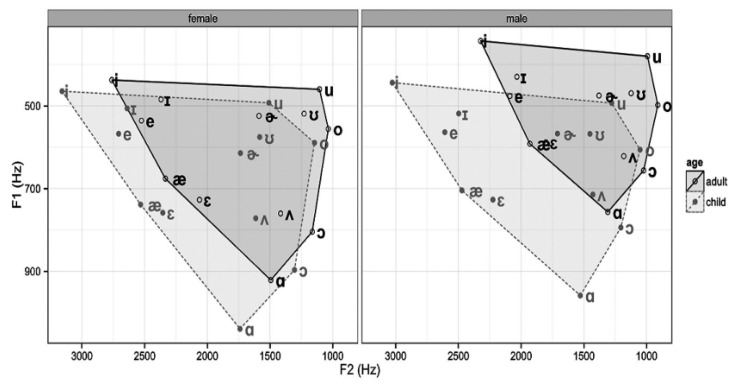
\includegraphics[scale=0.43]{vowel_space_comparison.jpg}
          \end{center}
        }
      \end{frame}

    \subsection{\subonethree}
      \begin{frame}[t]{\subonethree}
        \begin{definition}
          % Categorical perception
The general perceptual phenomenon in which discrete mental categories are created for non-discrete, variable stimuli

        \end{definition}
        \only<1>{
          \begin{center}
            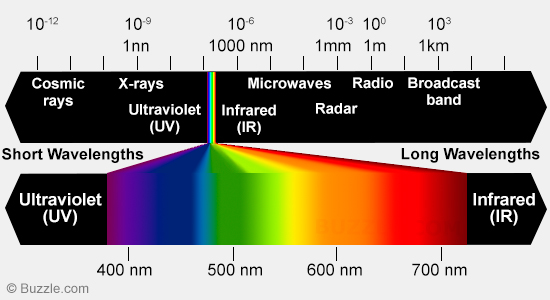
\includegraphics[scale=0.42]{color_spectrum.jpg}
          \end{center}
        }
        \only<2>{
          \begin{block}{What about in language?}
            \alert{Voice onset time} (VOT): % Voice onset time
The time between the release of a stop and the beginning of the voicing of the following vowel

            \begin{itemize}
              \item This is perceived categorically even though it is continuous
            \end{itemize}
          \end{block}
        }
        \only<3>{
          \begin{block}{For velar stops leading into [ɑ]}
            \begin{itemize}
              \item A VOT of 0ms is perceived as [ɡɑ]
              \item A VOT of 60ms is perceived as [kɑ]
            \end{itemize}
            But what about 20ms, 30ms, 40ms, etc.?
          \end{block}
        }
        \only<4>{
          \begin{columns}
            \column{0.48\linewidth}
              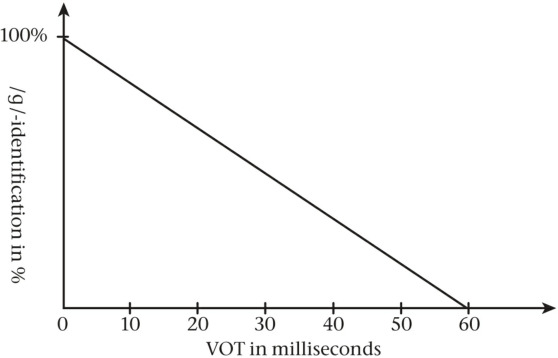
\includegraphics[scale=0.31]{vot_id_continuous.jpg}
            \column{0.48\linewidth}
              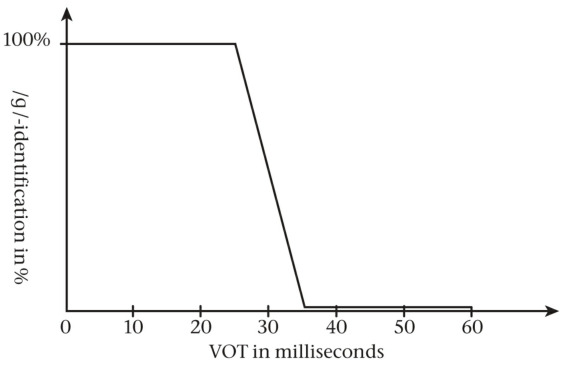
\includegraphics[scale=0.31]{vot_id_categorical.jpg}
          \end{columns}
        }
        \only<5>{
          \begin{block}{Super baby hearing}
            Six month old infants of English-speaking parents can discriminate between VOTs of 0ms and 20ms
            \begin{itemize}
              \item What does this tell us?
            \end{itemize}
          \end{block}
        }
        \only<6>{
          \begin{block}{Category boundaries differ between languages}
            \begin{itemize}
              \item VOT boundary for English speakers: 30ms
              \item VOT boundary for Spanish speakers: 20ms
            \end{itemize}
          \end{block}
        }
      \end{frame}

    \subsection{\subonefour}
      \begin{frame}{\subonefour}
        \begin{block}{Are the [k]s in \uttr{cool cat} the same?}
          \uncover<2->{
            The [k] in \lexi{cat} is advanced:
            \begin{itemize}
              \item \uttr{[k]ool [k̟]at}
            \end{itemize}
          }
        \end{block}
        \begin{alertblock}<2->{Coarticulation}
          % Coarticulation
The relationship between two adjacent sounds in which one has some effect on the quality of the other

        \end{alertblock}
        \begin{block}<2->{So how do we understand them?}
          \uncover<3->{
            Our perceptual system takes into account preceding and succeeding context and categorizes both as /k/
          }
        \end{block}
      \end{frame}

    \subsection{\subonefive}
      \begin{frame}{\subonefive}
        \begin{block}{}
          VOTs for faster speech are shorter and for slower speech are longer
        \end{block}
        \begin{block}{How do we manage to understand?}
          \uncover<2->{
            We normalize for the overall rate of speech
          }
        \end{block}
      \end{frame}

    \subsection{\subonesix}
      \begin{frame}{\subonesix}
        \begin{example}
          \href{https://youtu.be/aFPtc8BVdJk}{Which consonant do you hear?}
        \end{example}
        \begin{definition}<2->
          % McGurk effect
An illusion in which a visual of a speaker producing one sound is paired with audio of a different sound and a third sound is heard instead
 \parencite{mcgurk_hearing_1976}
        \end{definition}
        \begin{block}<2->{}
          \begin{itemize}
            \item The visual stimuli is consistent with [ɡ] and [d]
            \item The auditory stimuli is consistent with [b] and [d]
          \end{itemize}
          We use both to narrow down what we're hearing
        \end{block}
      \end{frame}

    \subsection{\suboneseven}
      \begin{frame}{\suboneseven}
        \begin{block}{We expect stimuli to match our mental grammars}
          If we're unsure of having heard [ʃk] or [sk], what do we do?
          \begin{itemize}
            \item<2-> Our phonotactics only allow [sk], so perceive [sk]
          \end{itemize}
        \end{block}
        \begin{block}<3->{We expect stimuli to match our mental lexicons}
          If we're unsure of having heard [ˈkɹin] or [ˈkrim], what do we do?
          \begin{itemize}
            \item<4-> {[}ˈkrim] is a word, so we perceive [m]
          \end{itemize}
        \end{block}
      \end{frame}

    \subsection{\suboneeight}
      \begin{frame}{\suboneeight}
        \begin{definition}
          % Phonemic restoration
The phenomenon in which listeners can fill in sounds in words that were not actually heard
 \parencite{warren_perceptual_1970}
        \end{definition}
        \begin{example}
          What is the utterance in \href{http://sites.sinauer.com/languageinmind/wa07.08.html}{the clip}?
        \end{example}
      \end{frame}

    \subsection{\subonenine}
      \begin{frame}{\subonenine}
        \begin{block}{Try these}
          \textcite{dawson_language_2016}, chapter 9 exercise 15
        \end{block}
      \end{frame}

      \begin{frame}{References}
        \printbibliography
      \end{frame}
\end{document}
